\chapter{Analysis}

\null\qquad After the set of parallelisability metrics has been devised and proposed (see chapter \ref{metrics}) and a working framework for metrics research and analysis has been implemented and set (chapter \ref{ppar-tool} describes developed PPar tool), software source code parallelisability metric values can be gathered and analysed. This analysis task in not that trivial. There is, principally, an unlimited number of ways in which this data can be visualized, interpreted and processed. This chapter describes analysis approaches and presents findings in the report. \newline
\null\qquad Table \ref{analysis-data-table} below presents the data, used for analysis. This data has been extracted from NAS parallel benchmarks (see chapter \ref{benchmarks}) and transformed into tabular format.
\begin{figure}[htb]
	\centering
	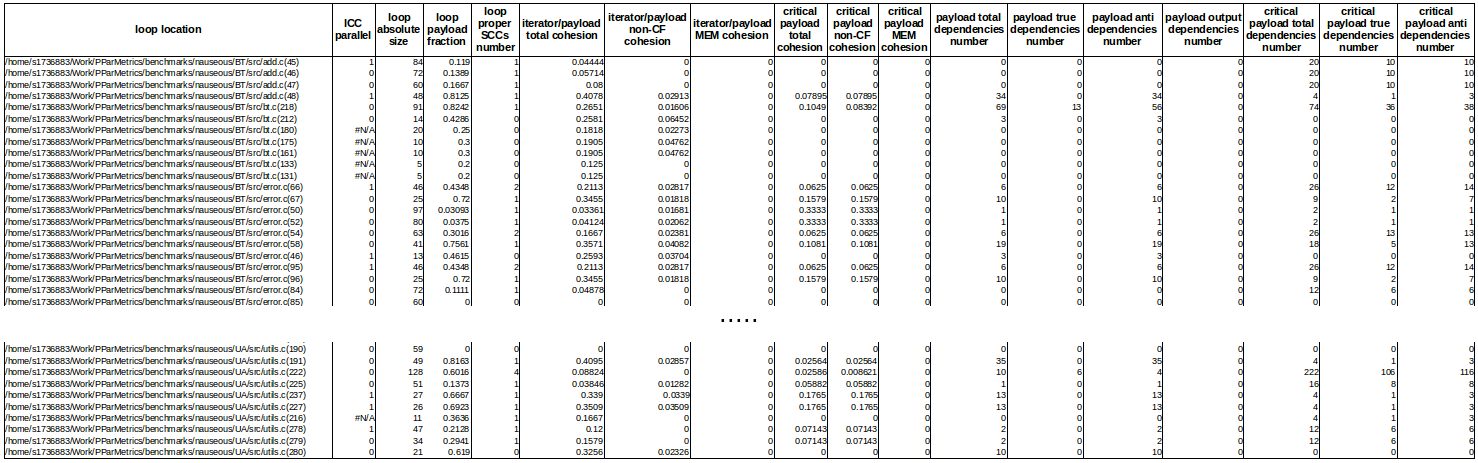
\includegraphics[width=\linewidth]{figs/metrics-table.png}
	\caption{Analysis input table with computed metrics and ICC parallelizability classification labels.}
	\label{analysis-data-table}
\end{figure} \newline
\null\qquad This data is, essentially, a set of loops found in NAS benchmarks. For every single loop a vector of metrics (loop features) has been computed. All loops have passed through Intel C/C++ compiler parallelisability analyses and have been classified (labelled) as parallelizible or not. ICC compiler plays a role of expert in this project. The table \ref{analysis-data-table} contains around 1400 loops with and 13-dimensional feature vector for each. \newline 
\null\qquad This dataset has been analysed in several ways. First, the collected data has been visualized to see if there are any obvious correlations between loop parallelisability and metric values. Section \ref{analysis-data-interpretation-and-visualization} presents these visualizations and describes all found corerlations. This visualization has been done for every single metric (seen subsection) as well as for the whole set of metrics altogether (see subsection). To visualize the whole combined set of metrics Principal Component Analysis (PCA) and clustering techniques have been used. Section \ref{analysis-manual-analysis} supplements these visualizations with some manually derived insights into analysis results. \newline 
\null\qquad Then, statistical analysis techniques have been applied to the data. Loop metrics have been viewed as machine learning features in the context of loop parallelisability classification problem. Standard state-of-the-art  machine learning techniques (such as Support Vector Machines (SVM), desicion trees, etc) have been applied to the data and all prediction errors have been compared agains random predictor. Section \ref{analysis-statistical-analysis} presents a report on this. \newline
\null\qquad There has already been an attempt to apply statistical analysis techniques to see how software quality metrics, such as cyclomatic complexity \ref{background-cyclomatic-complexity} and Halstead's software science measures \ref{background-halsteads-measures} behave on Mozilla Firefox browser and LLVM compiler components library open source codes \cite{source-code-quality-classification-paper}. Authors applied k-means clustering and got 3 clusters of software quality metric values for subroutines. But there were no classifications attached to the input data and no correlations have been examined. There could easily be subroutines of different software quality grades in the same cluster. \newline
\null\qquad All results have been derived thanks to Python programming language and its packages: pandas \cite{python-lib-pandas}, matplotlib \cite{python-matplotlib} and scikit-learn \cite{python-lib-scikit-learn}. 

\section{Analyses preparation phase}
\label{analysis-preparation-phase}
\qquad Before we move onto the actual description of gathered results, there is a need to describe some preparatory data preprocessing procedures, which have been used throughout all analysis stages. \newline  
\null\qquad As it turned out, there are some outliers in the collected data that distort the final result. For example, figure \ref{outliers-filtering} shows the plot of payload total dependencies number metric values on all NAS benchmark loops. The plot on the left shows metric values dispersion before outliers elimination. It can be seen that there is a non-parallelizible (red dot) loop with almost 12000 dependencies in the payload which seriously shifts mean metric values for parallelizible and non-parallelizible subsets to the point of correlation inversion. Generally, it makes sense that the more dependencies we have in the payload, the harder it has to be to parallelize the loop. And it is seen from the whole dataset that loops with really high dependencies numbers have not been parallelized by the ICC compiler. But for majority of loops, encountered in NAS benchmarks, this tendency does not take place. Right plot contains only those loops, which have metric values withing 3 standard deviations from the mean. Here ICC parallelization ability does not really correlate with the amount of dependencies in the payload of the loop. The total number of dependencies in the payload of a loop is not the only metric, where we have some outliers. Similar filtering measures have been taken for all metrics.   
\begin{figure}[h]
\centering
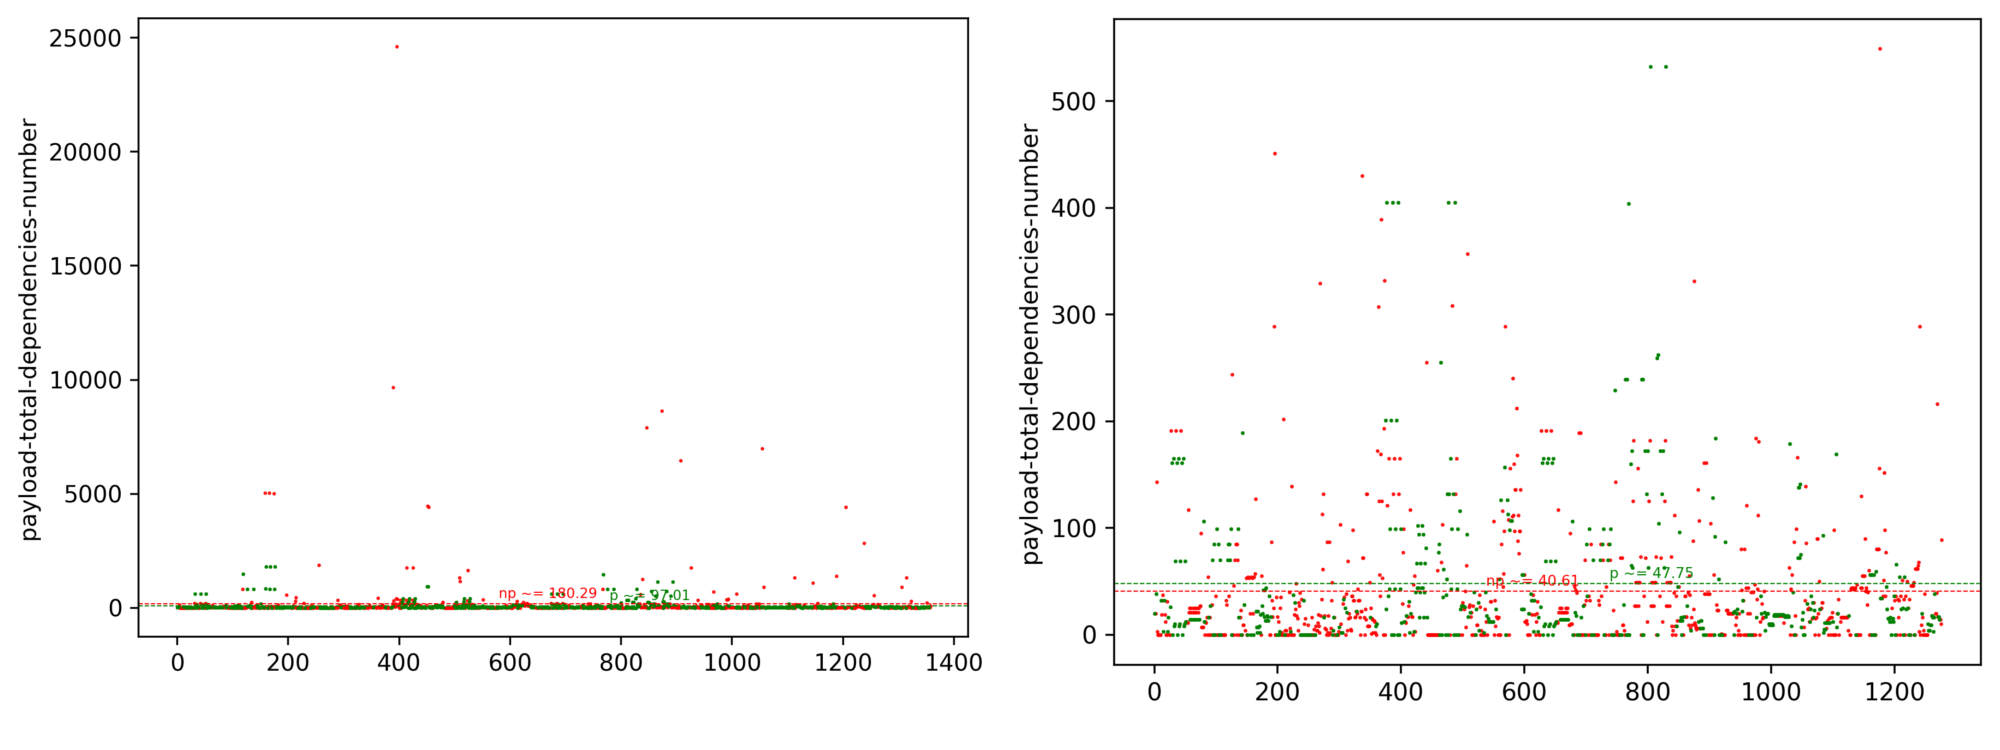
\includegraphics[width=\linewidth]{figs/outliers-filtering.png}
\caption{Distribution of total dependencies number metric values on all NAS benchmark loops before and after elimination of all cases beyond 3 standard deviations from the mean.}
\label{outliers-filtering}
\end{figure} \newline 
\null\qquad There was also a need to normalize the data before application of Principal Component Analysis (PCA) algorithm, in order to make a better graphical visualization.

\section{Data interpretation and visualization}
\label{analysis-data-interpretation-and-visualization}
\subsection{Single loop metrics vs loop parallelisability analysis}
\qquad The layout of this section corresponds to that of section \ref{metrics-metric-groups}, which describes proposed groups of software parallelisability metrics. Subsections below present their parallelizability correlation results.  
\subsubsection{Loop proportion metrics}
\label{analysis-loop-proportion-metrics}
\qquad Figures \ref{loop-proportions-0} and \ref{loop-proportions-1} present plots of loop proportion metric values, gathered on all NAS benchmark loops. All outliers lying beyond 3 standard deviations have been filtered (see section \ref{analysis-preparation-phase}). 
\begin{figure}[htb]
\centering
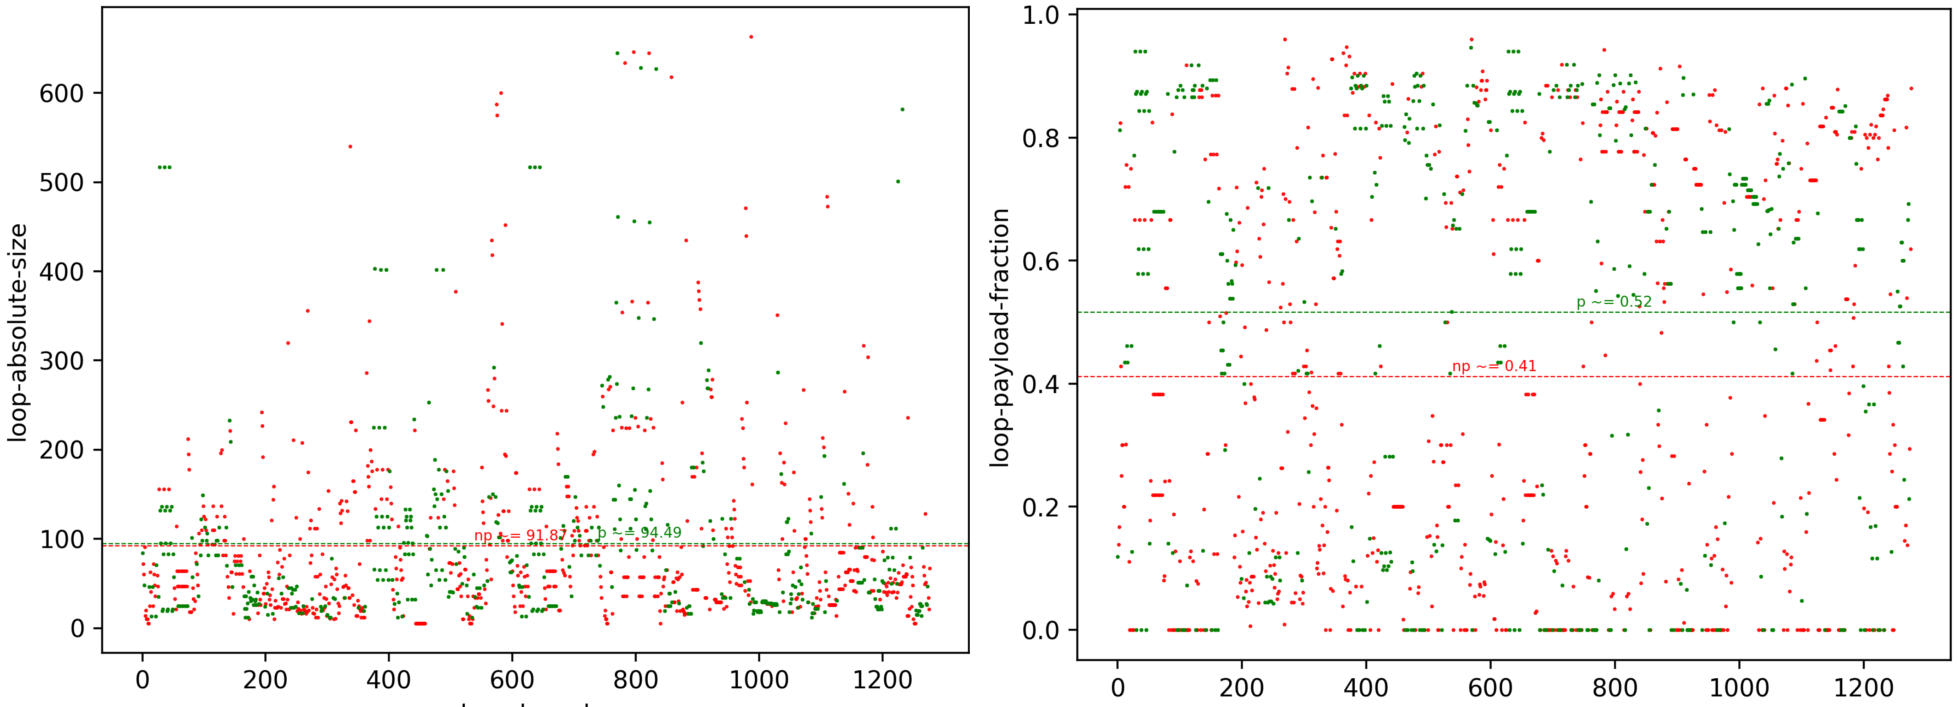
\includegraphics[width=\linewidth]{figs/loop-proportions-0.png}
\caption{\textit{Loop absolute size} metric on the left and \textit{loop payload fraction} metric on the right. Red and green dots represent loops, which have not/have been parallelized by ICC compiler correspondingly.}
\label{loop-proportions-0}
\end{figure}
\begin{figure}[htb]
\centering
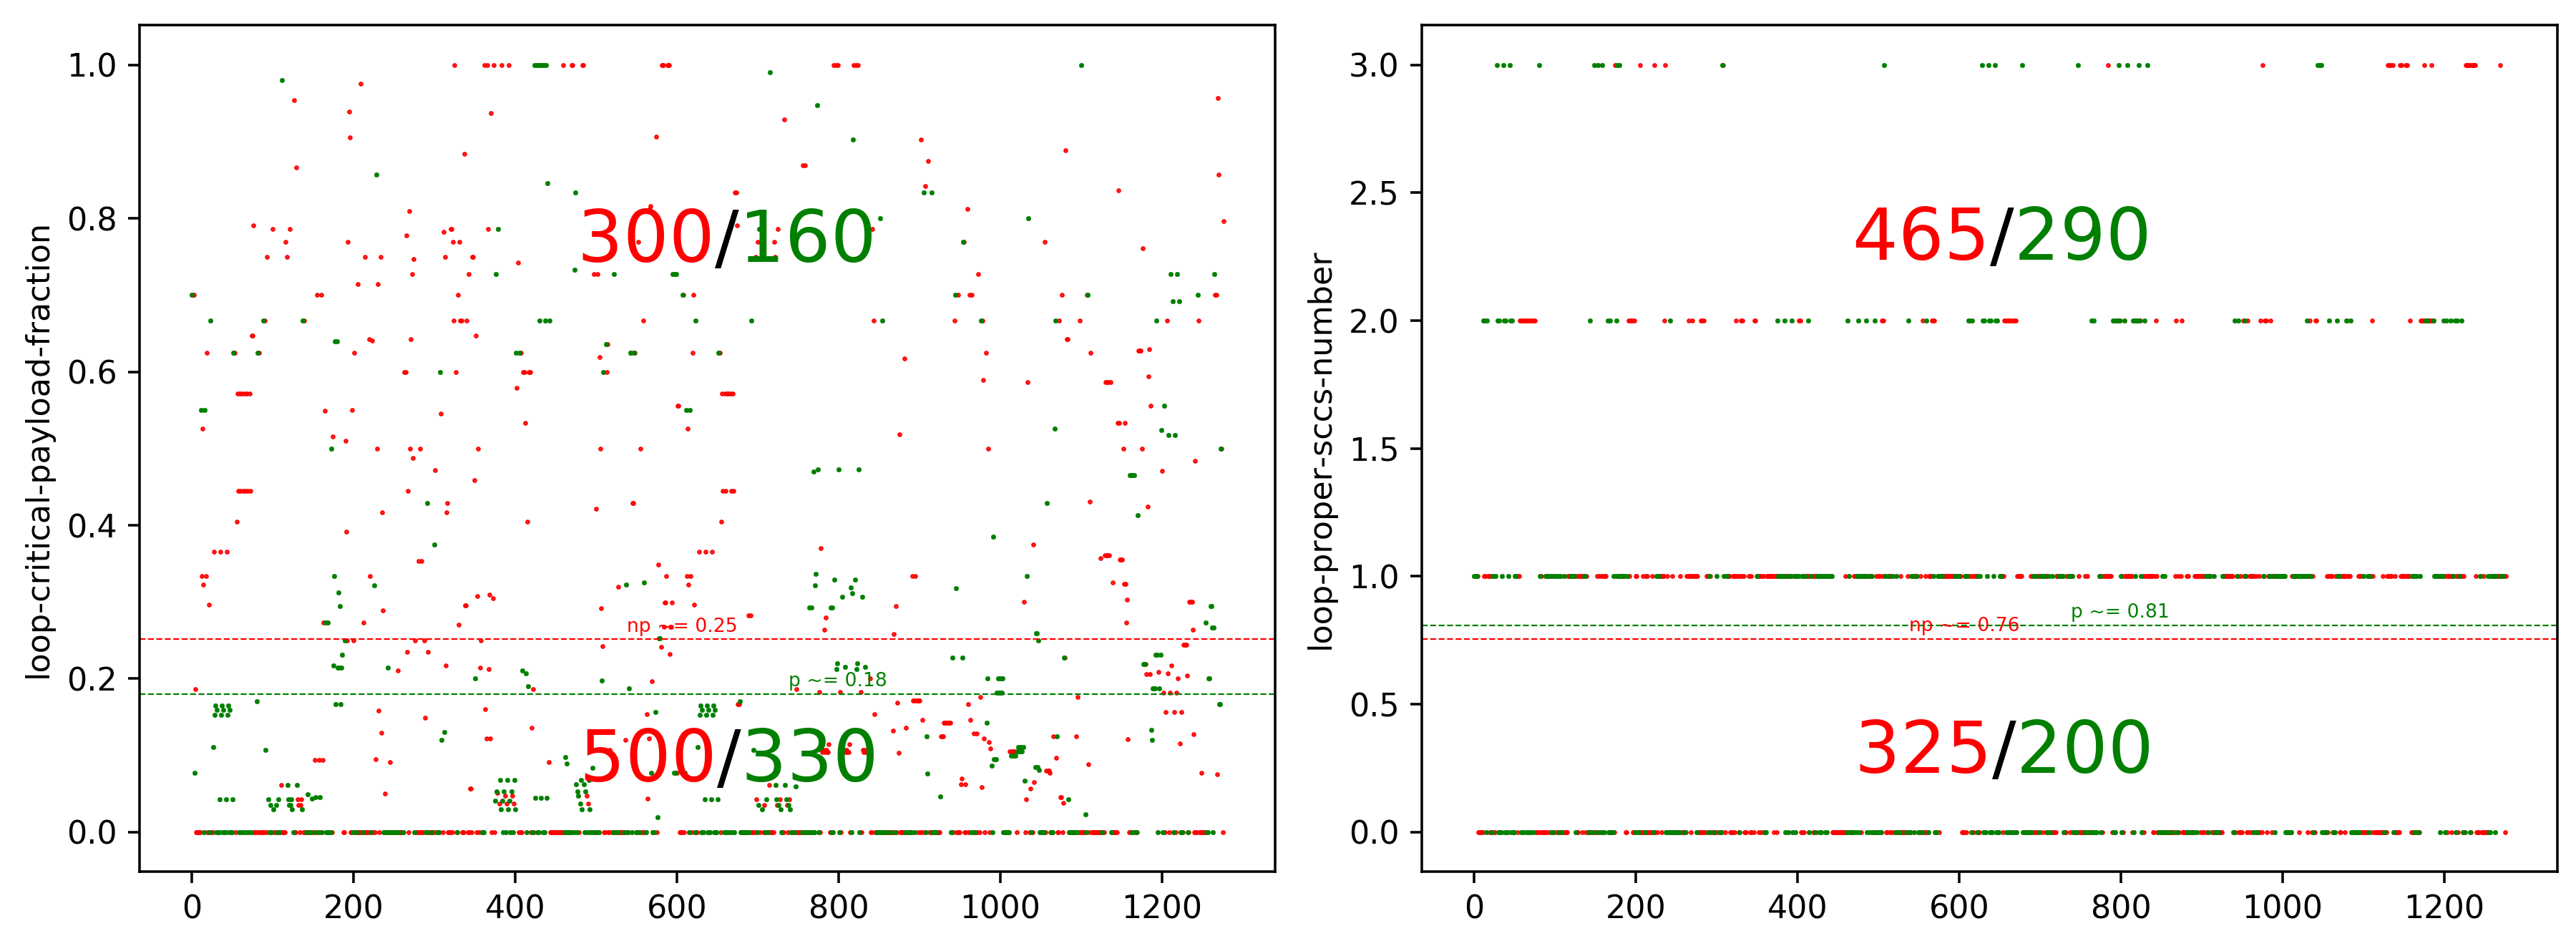
\includegraphics[width=\linewidth]{figs/loop-proportions-1.png}
\caption{\textit{Loop critical payload fraction} metric on the left and \textit{loop proper SCCs number} metric on the right. Red and green dots represent loops, which have not/have been parallelized by ICC compiler correspondingly.}
\label{loop-proportions-1}
\end{figure} \newline
\null\qquad As it can be seen from the plots, \textit{loop absolute size} does not really correlate with ICC parallelization ability. It must be clear from the nature of the metric. Size by itself does not prohibit loop parallelization. There might be a big loop with no cross-iteration dependencies, which must have a big portion of parallelism and should bring huge overall performance gains with its parallelization. \newline
\null\qquad There is pretty noticeable correlation between loop parallelisability and values of \textit{loop payload fraction} metric. Green dots are scattered predominantly at the top of the plot. The bigger the payload of a loop in comparison with its iterator, the more seducing this loop for compiler to parallelize. Bigger payloads bring better performance gains with parallelization. Another consideration might also be applied here. Bigger iterators are common for loops, which, for example, perform traversal of more complex data structures like linked-lists or alike. Such loops contain memory operations linking iterator and payload - \textit{iterator payload memory cohesion} metric should be non zero for such loops. Unfortunately, thare are no such loops in NAS benchmark set and the latter metric has been excluded from consideration at all. \newline 
\null\qquad Despite the fact that \textit{loop proper SCCs number} metric does not correlate with loop parallelizability that much, another metric of the same essense shows pretty good correlations. \textit{Loop critical payload fraction} metric can be used to judge about loop parallelizability. Connection between this metric and parallelizability property follows just out of common sense. Critical payload parts represent strongly connected components with more than one instructions. There are graph loops with forward and back edges inside such SCCs. Usually it happens when two memory instructions reference the same location on different (or the same) loop iterations and introduce 2 inverse-directed edges with anti and true dependencies. Such critical loop payload parts introduce actual parallelization constraints. The left plot in the figure \ref{loop-proportions-1} illustrates this connection. The bigger the critical component in the payload, the harder it is to parallelize the loop.        

\subsubsection{Loop Dependence Metrics}
\label{analysis-loop-dependence-metrics}
\qquad Figures \ref{loop-dependencies-number-0}, \ref{loop-dependencies-number-1} and \ref{loop-dependencies-number-2} present plots of loop dependencies number metric values. These metrics do not seem to be particularly reliable, when it comes to judging about loop parallelizability.  
\begin{figure}[h]
\centering
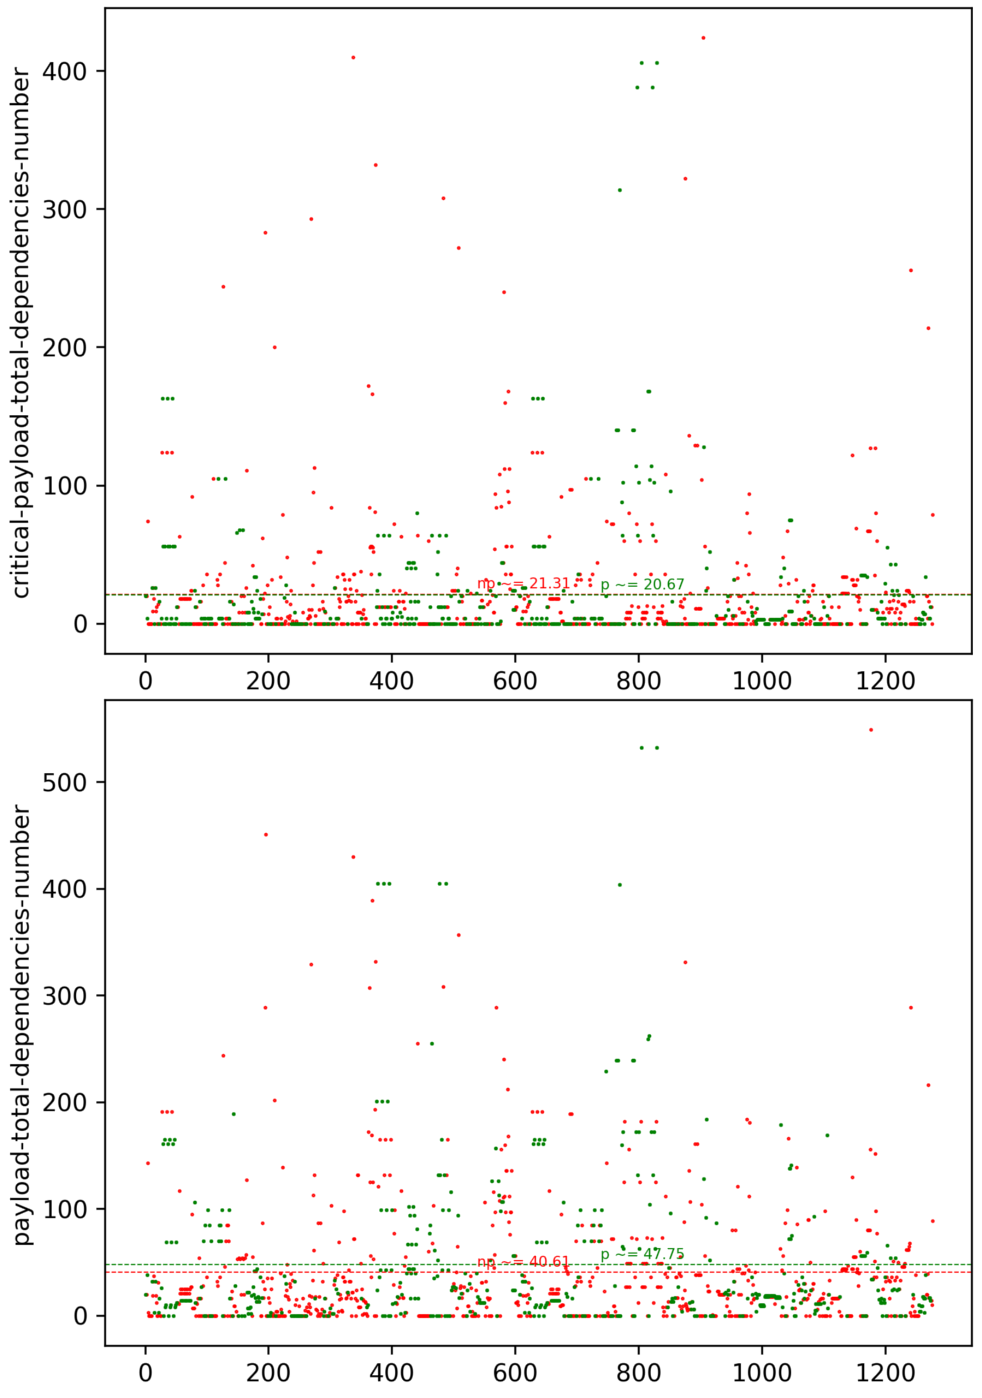
\includegraphics[width=\linewidth]{figs/loop-dependencies-number-0.png}
\caption{\textit{Critical payload dependencies number} metric on the left and \textit{total payload dependencies number} metric on the right. Red and green dots represent loops, which have not/have been parallelized by ICC compiler correspondingly.}
\label{loop-dependencies-number-0}
\end{figure}
\begin{figure}[h]
\centering
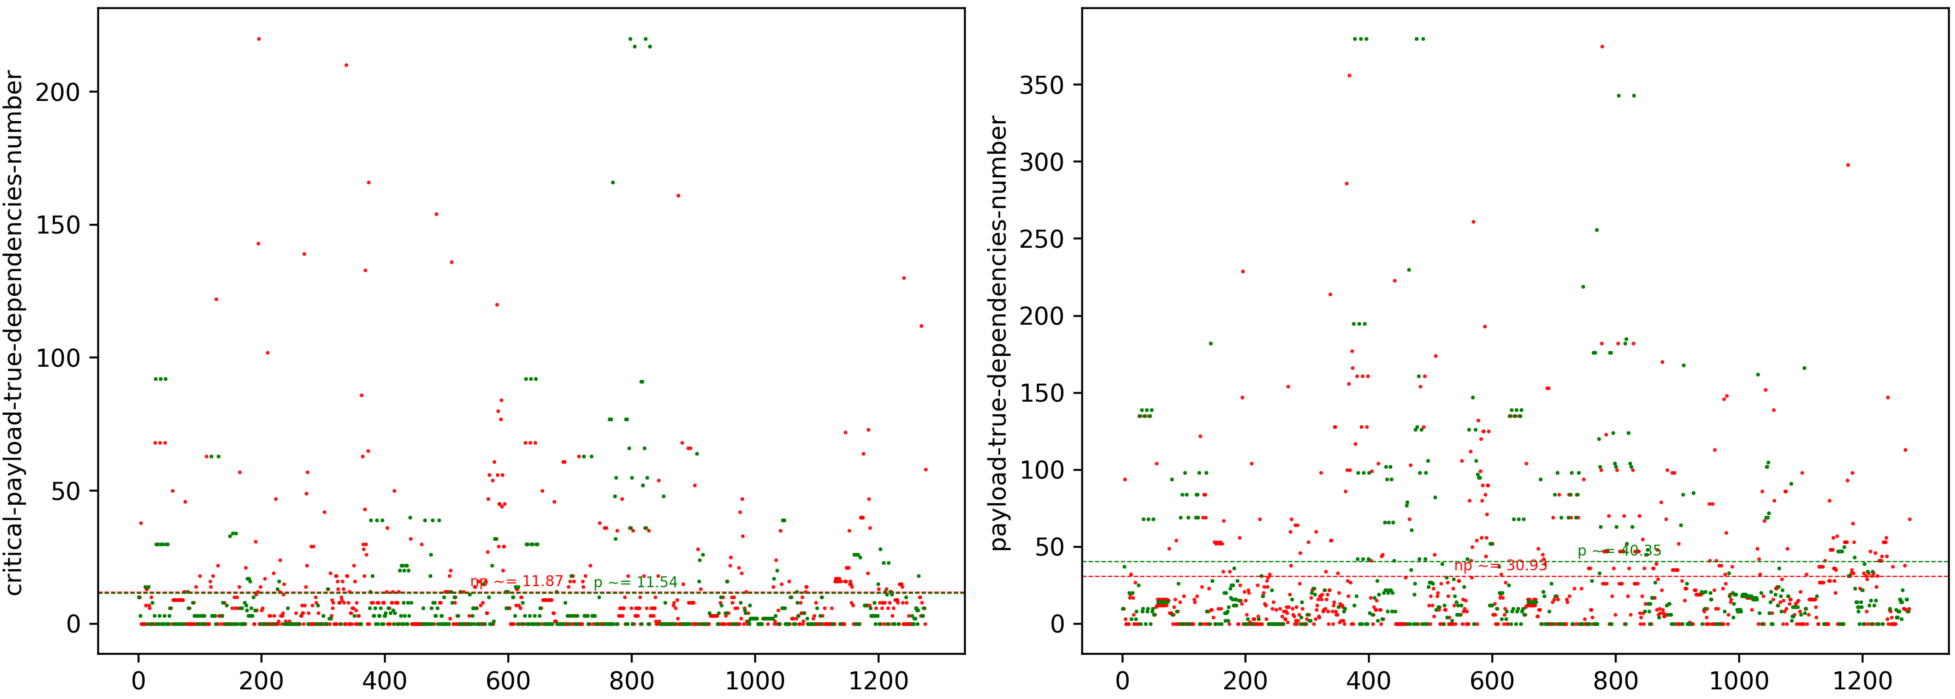
\includegraphics[width=\linewidth]{figs/loop-dependencies-number-1.png}
\caption{\textit{Critical payload true dependencies number} metric on the left and \textit{payload true dependencies number} metric on the right. Red and green dots represent loops, which have not/have been parallelized by ICC compiler correspondingly.}
\label{loop-dependencies-number-1}
\end{figure}
\begin{figure}[h]
\centering
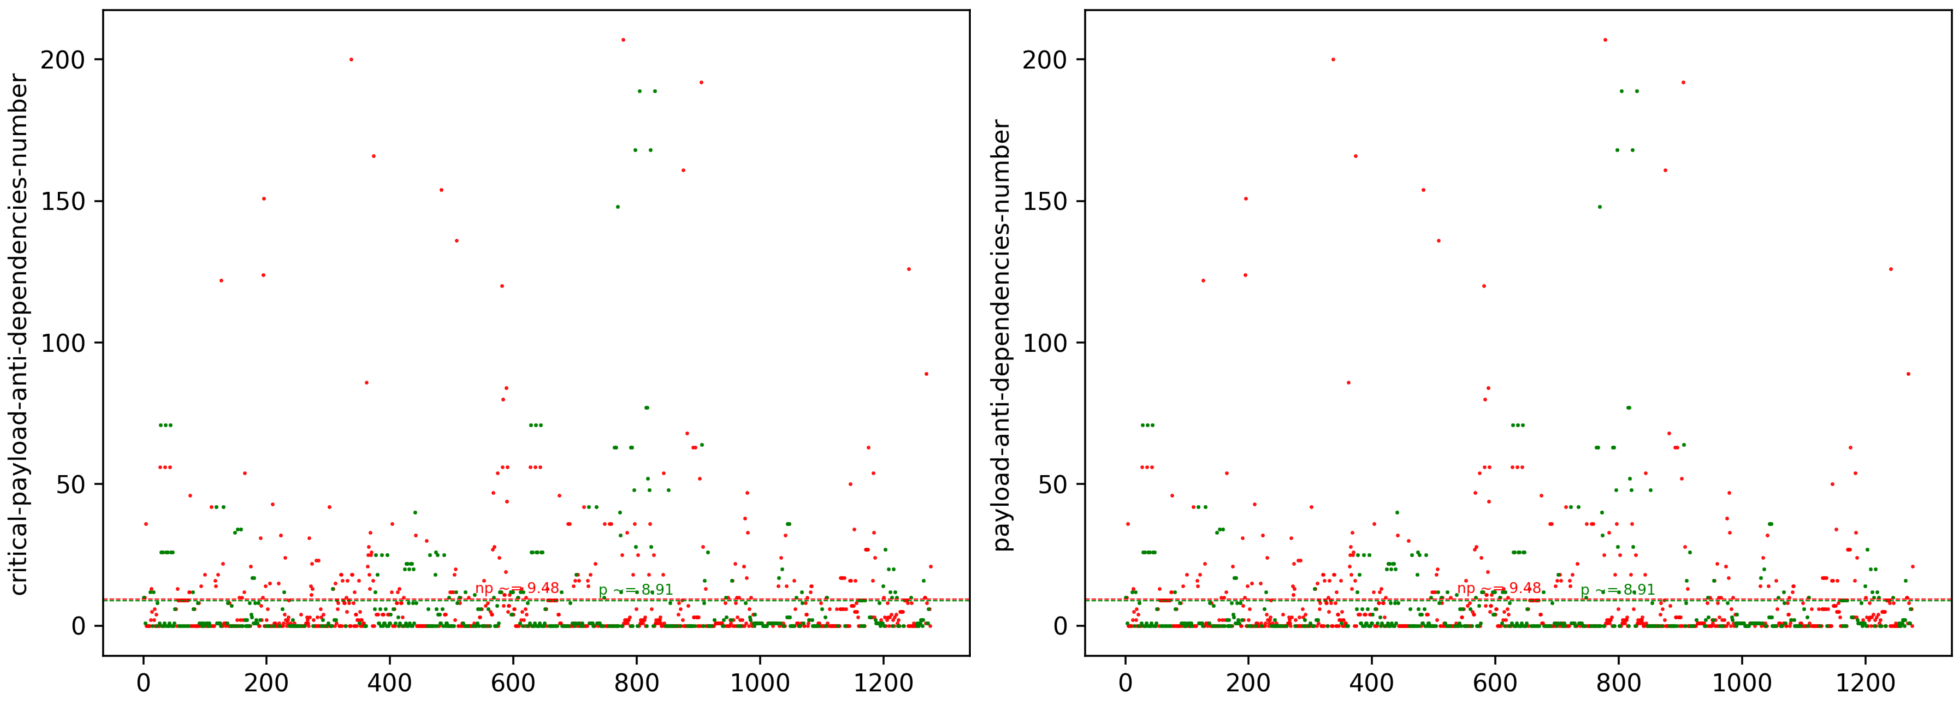
\includegraphics[width=\linewidth]{figs/loop-dependencies-number-2.png}
\caption{\textit{Critical payload anti dependencies number} metric on the left and \textit{payload anti dependencies number} metric on the right. Red and green dots represent loops, which have not/have been parallelized by ICC compiler correspondingly.}
\label{loop-dependencies-number-2}
\end{figure} \newline
\null\qquad These metrics 

\subsubsection{Loop Cohesion Metrics}
\label{analysis-loop-cohesion-metrics}
\qquad Figures \ref{loop-cohesion-0} and \ref{loop-cohesion-1} present plots of loop cohesion metric values.   
\begin{figure}[h]
\centering
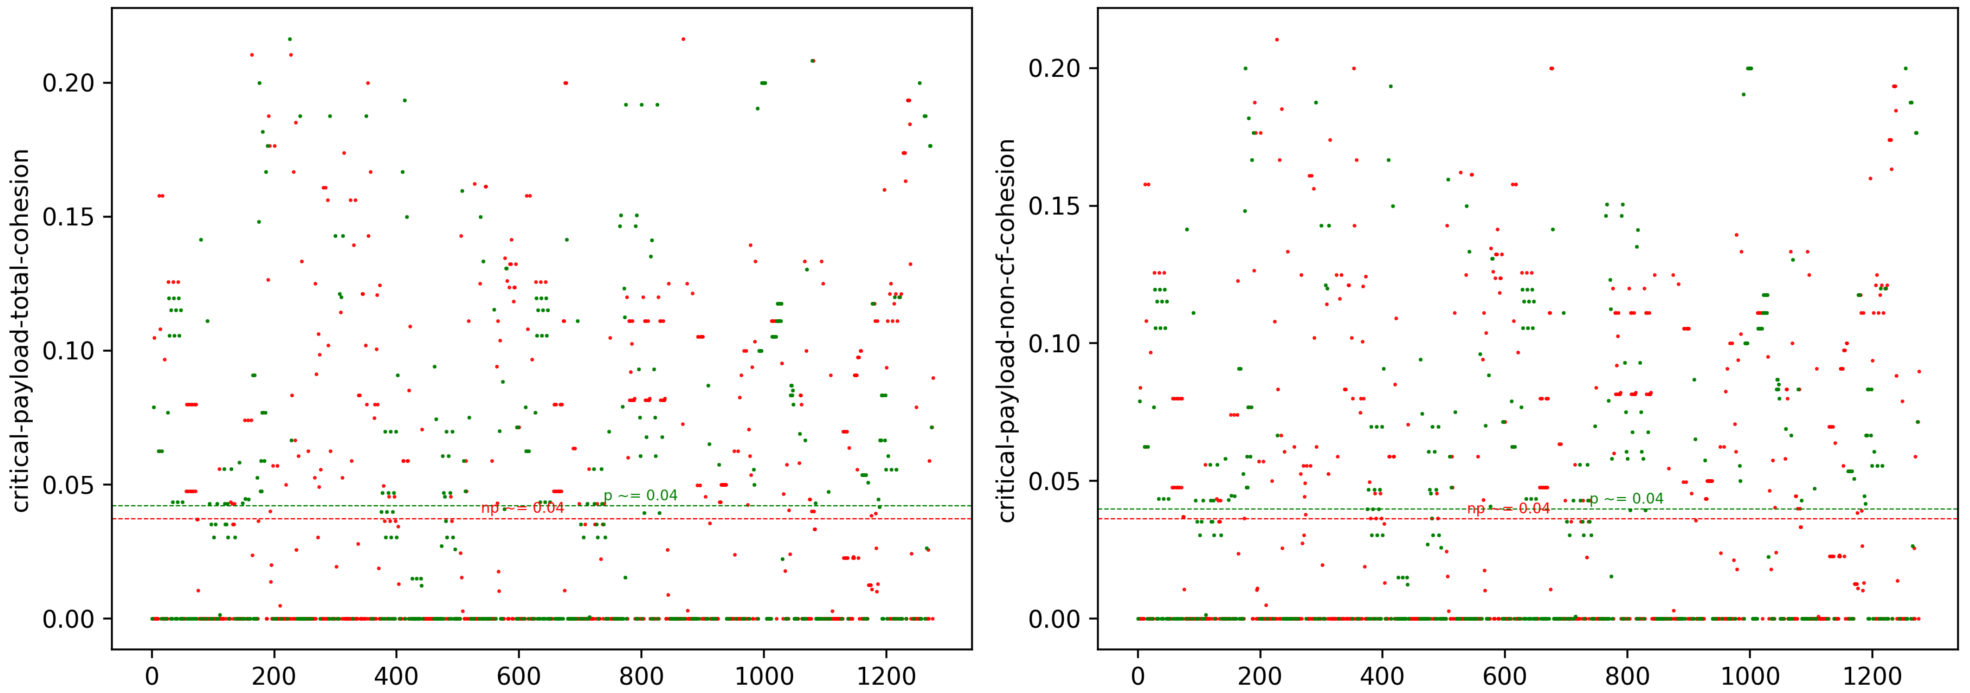
\includegraphics[width=\linewidth]{figs/loop-cohesion-0.png}
\caption{\textit{Critical payload total cohesion} metric on the left and \textit{critical payload non-cf cohesion} metric on the right. Red and green dots represent loops, which have not/have been parallelized by ICC compiler correspondingly.}
\label{loop-cohesion-0}
\end{figure}
\begin{figure}[h]
\centering
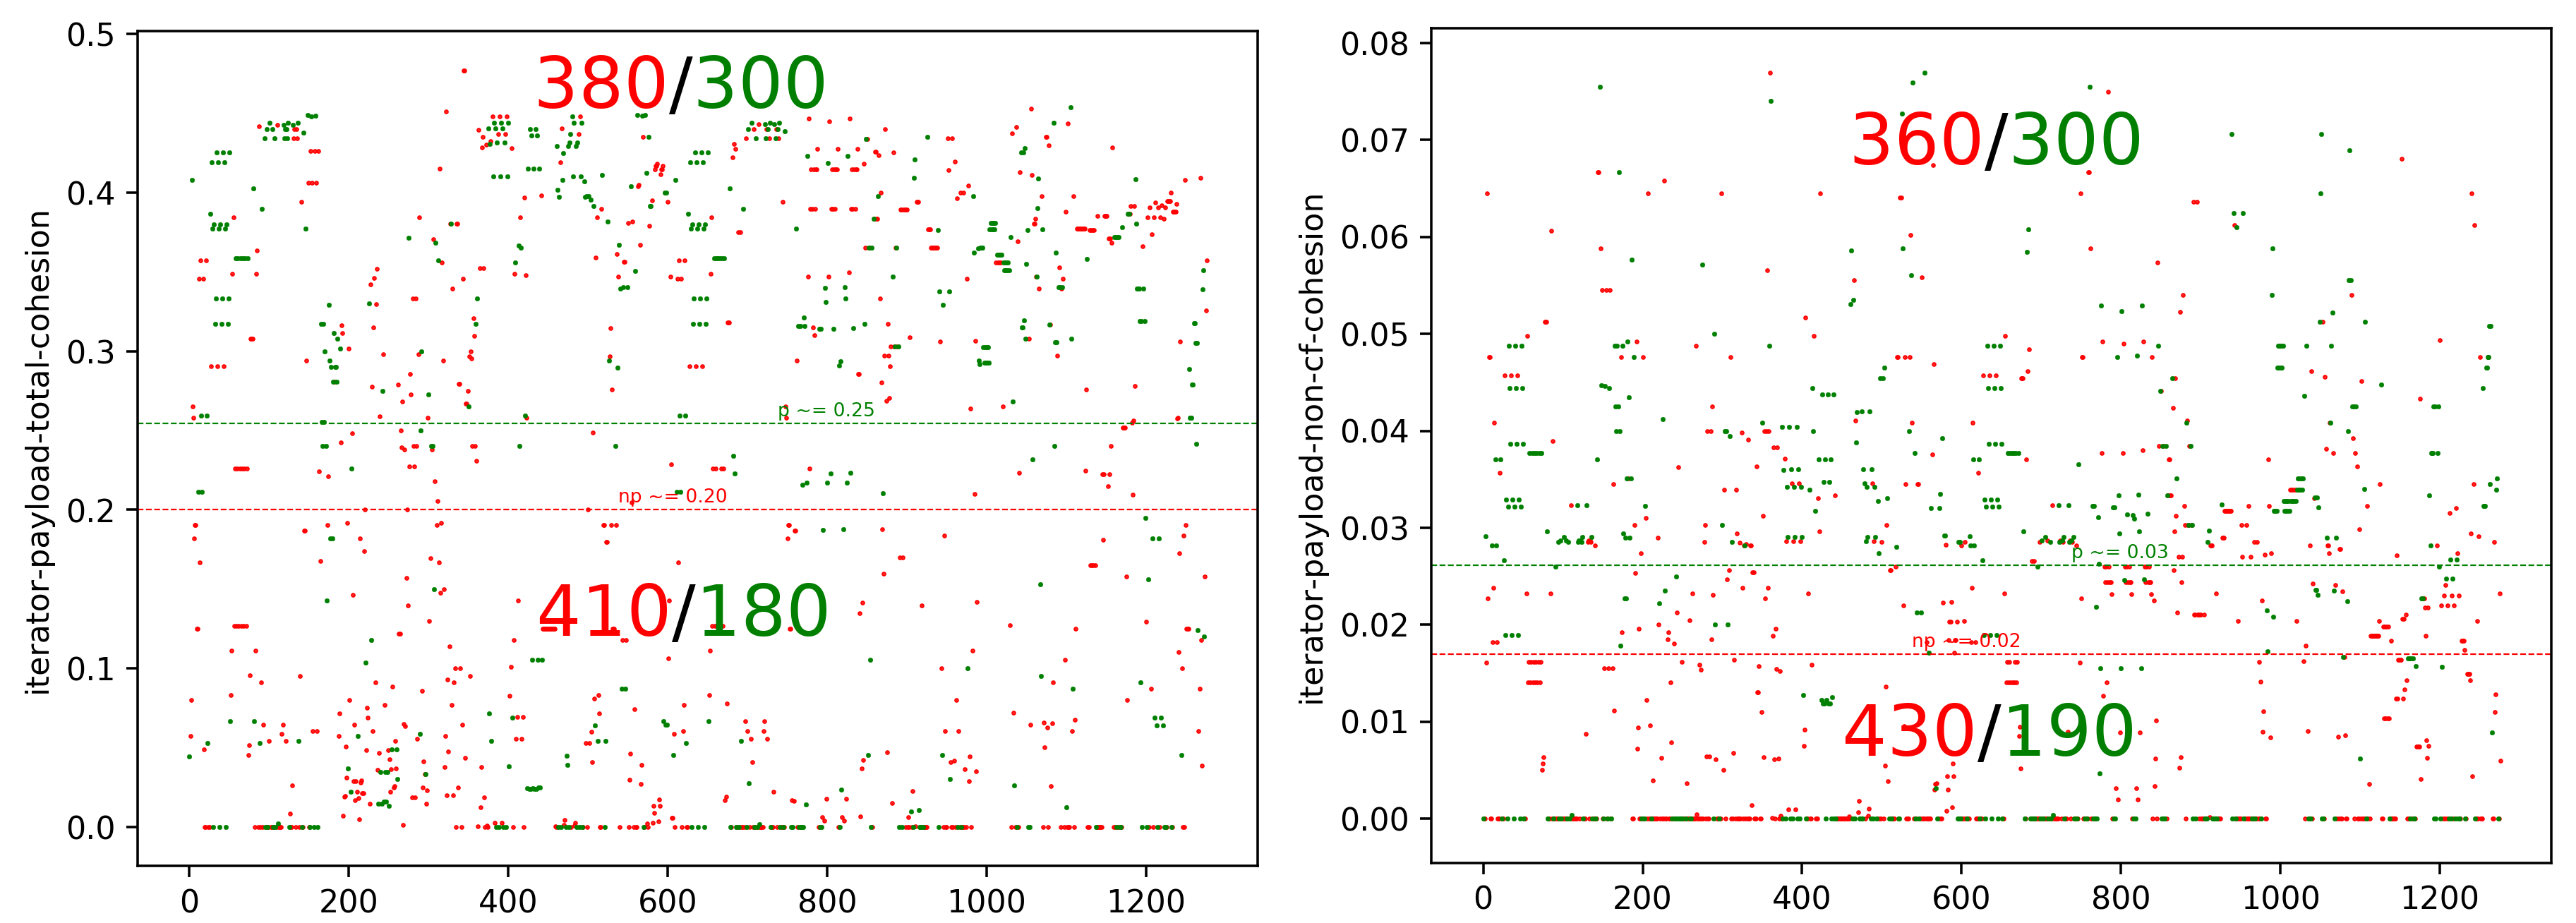
\includegraphics[width=\linewidth]{figs/loop-cohesion-1.png}
\caption{\textit{Iterator payload total cohesion} metric on the left and \textit{Iterator payload non-cf cohesion} metric on the right. Red and green dots represent loops, which have not/have been parallelized by ICC compiler correspondingly.}
\label{loop-cohesion-1}
\end{figure}
\subsection{Data clustering analysis}
\label{analysis-data-clustering-analysis}
\qquad This section describes the results of dataset clustering analysis. Data from the table \ref{analysis-data-table} can be viewed as a set of 13-dimensional vectors, describing NAS benchmark loops. For every loop, thanks to Intel C/C++ compiler, we know the right answer regarding its parallelisability. This section reports studies about correlations between spatial and structural properties of these vectors and parallelisability properties.    

\subsection{Combined metrics dataset visualization}
\label{analysis-data-clustering-analysis}
\qquad This section describes an attempt to conduct structural data analysis and identify separate clusters in the data. Since loops are represented by 13-dimensional vectors, direct dataset visualization is unfeasible. Principal Components Analysis (PCA) has been used to project the data onto 3-dimensional space and visualize it. Figure \ref{metrics-pca-13-to-3} provides an illustration of distribution of metric values on all loops. It is visible from the figure, that data values do not form any apparent clusters, but there are some areas of increased density though.
\begin{figure}[htb]
\centering
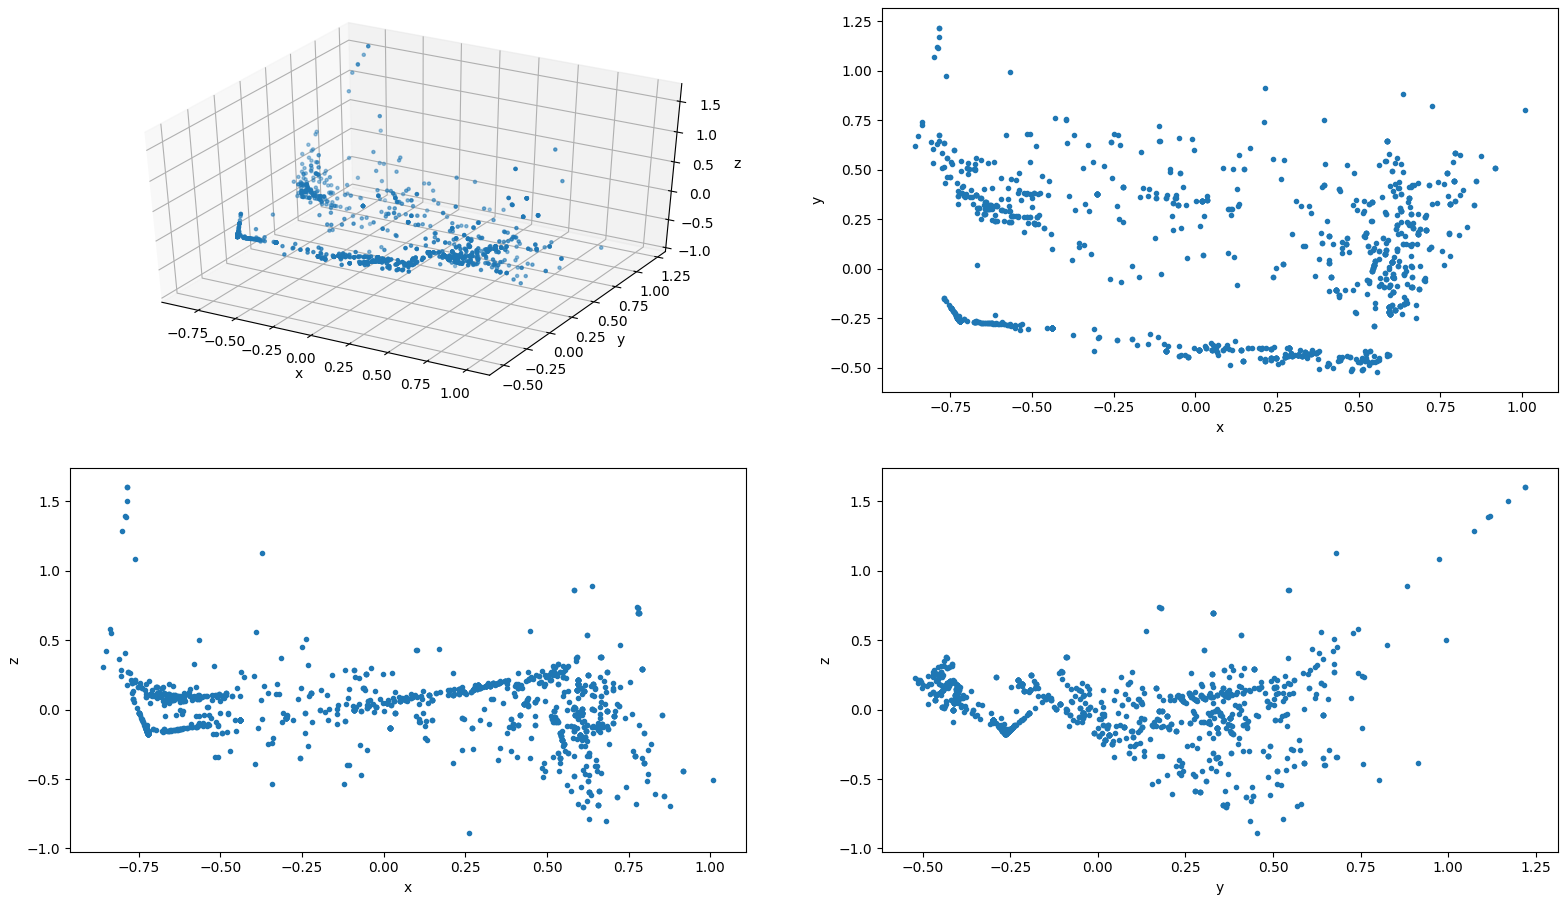
\includegraphics[width=\linewidth]{figs/metrics-pca-13-to-3.png}
\caption{Visualisation of loop metrics dataset spatial distribution (13-dimensional metric vectors have been projected onto 3D space thanks to PCA algorithm) - blue dots correspond to metric values of single loops.}
\label{metrics-pca-13-to-3}
\end{figure} \newline 
\null\qquad Metric dataset projection onto 2D plane looks alike XY projection of 3D PCA mapping (see figure \ref{metrics-pca-13-to-2}). \newline
\null\qquad Next step is to establish correlation between structural properties of dataset distribution and loop parallelizability. Figure \ref{metrics-pca-parallelizability} provides an illustration for it. Out of that figure it is visible that there is no apparent correlation between combined metric values and parallelizability of loops these metrics represent. 
\begin{figure}[htb]
\centering
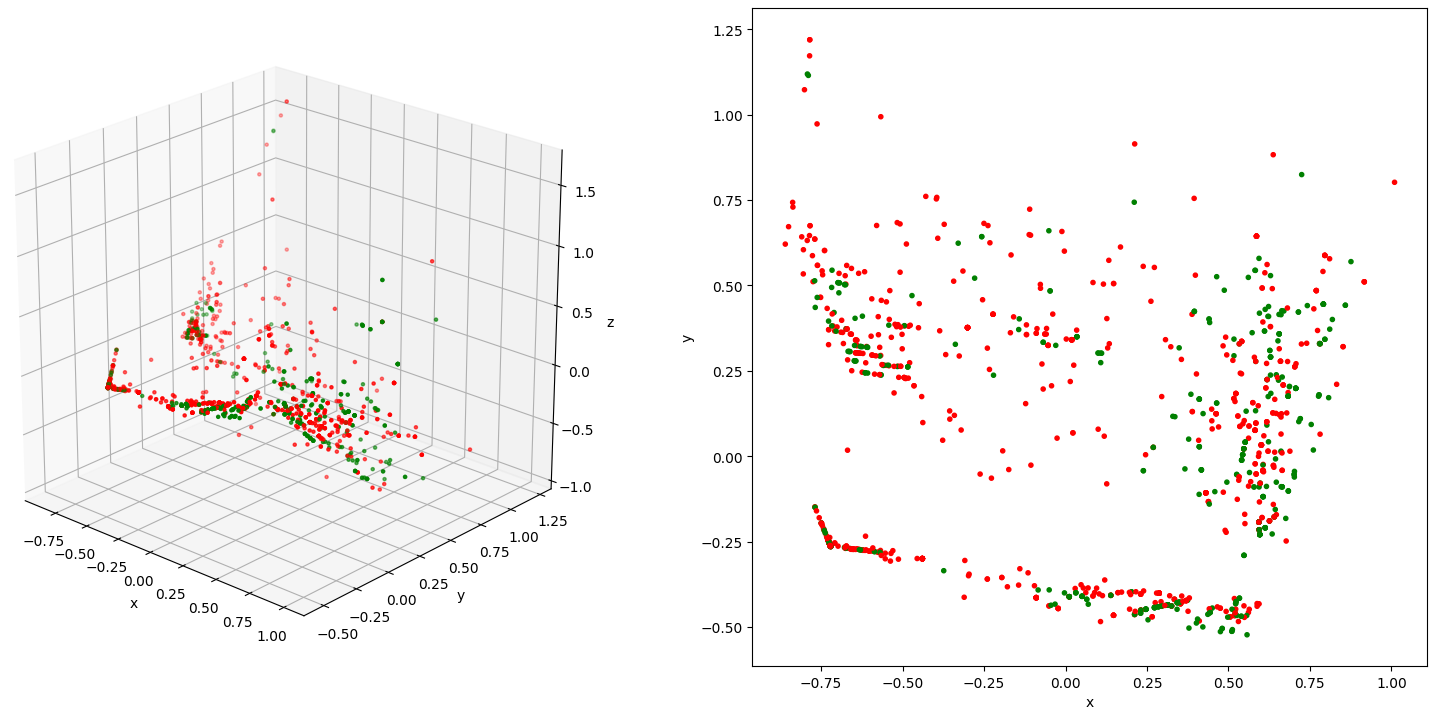
\includegraphics[width=\linewidth]{figs/metrics-pca-parallelizability.png}
\caption{Visualisation of loop metrics dataset spatial distribution (3D PCA projection on the left, 2D PCA projection on the right) versus parallelizability property. Red dots - non-parallelizible loops; green dots - parallelizible loops}
\label{metrics-pca-parallelizability}
\end{figure} \newline
\null \qquad It would be interesting to see, what kind of loops and metric values form these areas of increased density. To get that information we can apply k-means clustering algorithm and get subsets of loops, which form these condensed clots. We need to pick the number of clusters. The number of clusters might be arbitrary, but from the figure it is visible that 3 or 4 clusters would be quite a close approximation to the given dots distribution. Figure \ref{metrics-4-clusters} illustrates the results of k-means clustering algorithm run with 4 clusters. Algorithm has almost perfectly identified the structure of dots distribution. Maybe yellow and blue subsets must be in the same subset. We can consider all these blue and yellow loops altogether. Some dots (the ones on the boundary of red cluster) also happened to be blue, while red classification would be the most appropriate for them. To exclude these must-be-red blue loops from considerations applied to the blue cluster, euclidean distances from cluster centers were computed for every dot. Only loops near cluster centers are considered in the manual source code study. Table \ref{clusters-metric-values} presents average values for all metrics in 4 clusters. \newline
\null\qquad 

\begin{figure}[htb]
\centering
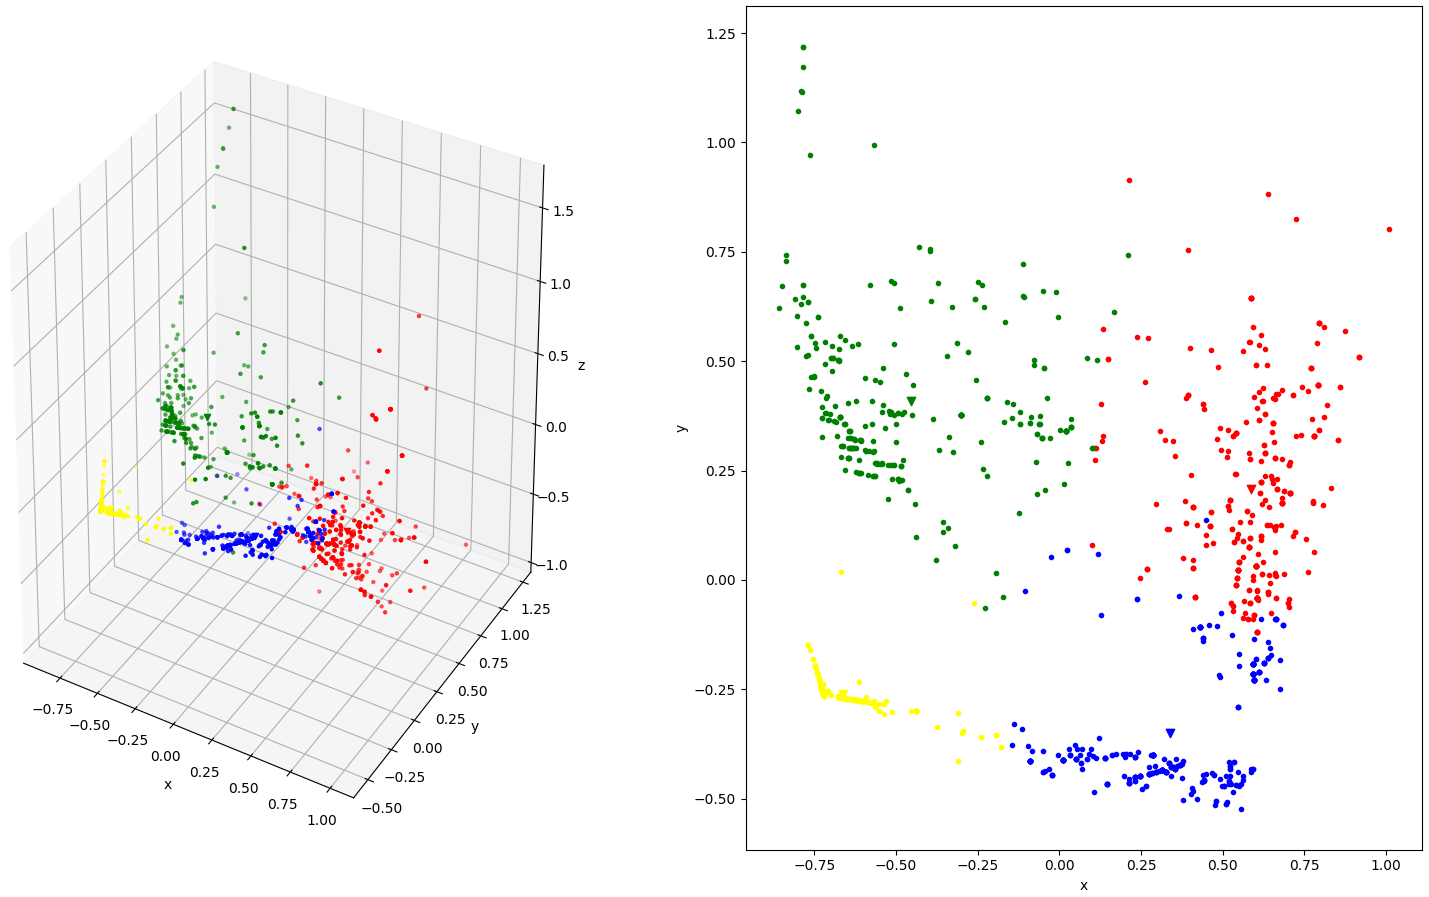
\includegraphics[width=\linewidth]{figs/metrics-4-clusters.png}
\caption{k-means algorithm classified the dataset into 4 separate clusters.}
\label{metrics-4-clusters}
\end{figure}

\begin{figure}[htb]
\centering
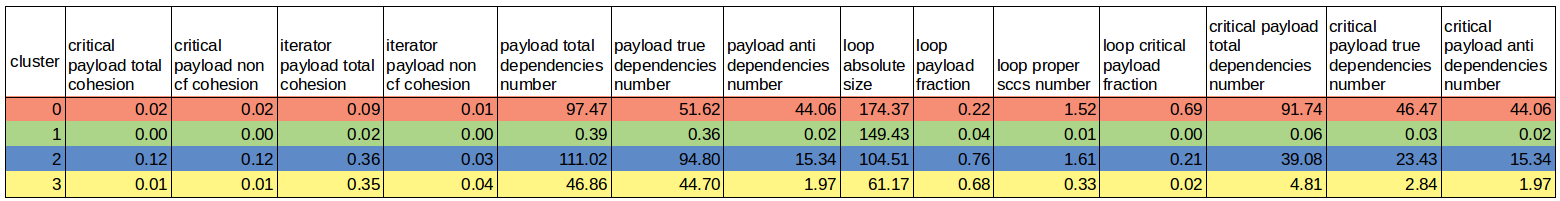
\includegraphics[width=\linewidth]{figs/clusters-metric-values.png}
\caption{Average metric values for 4 different clusters}
\label{clusters-metric-values}
\end{figure} 

\section{Manual analysis}
\label{analysis-manual-analysis}

\subsection{The problem of proper SCCs number metric}
\qquad The proper SCCs number metric was described in section \ref{metrics-loop-proper-sccs-number}. Despite the fact, that the metric seems to directly represent parallelisability inhibiting parts of the payload, figures in ... show that ICC compiler sometimes fails to parallelise loops even with 0 metric value. Listing \ref{lst:metrics-loop-example-2} below, gives such example.

\begin{lstlisting}[caption={Non-parallelizible loop. Function call inside loop's body prevents ICC compiler from parallelizing it. Loop taken from EP NAS benchmark.}, captionpos=b, label=lst:metrics-loop-example-2, float,floatplacement=H]
for (i = 0; i < MK + 1; i++) {
	t2 = randlc(&t1, t1);
}
\end{lstlisting}

\begin{figure}[htb]
	\centering
	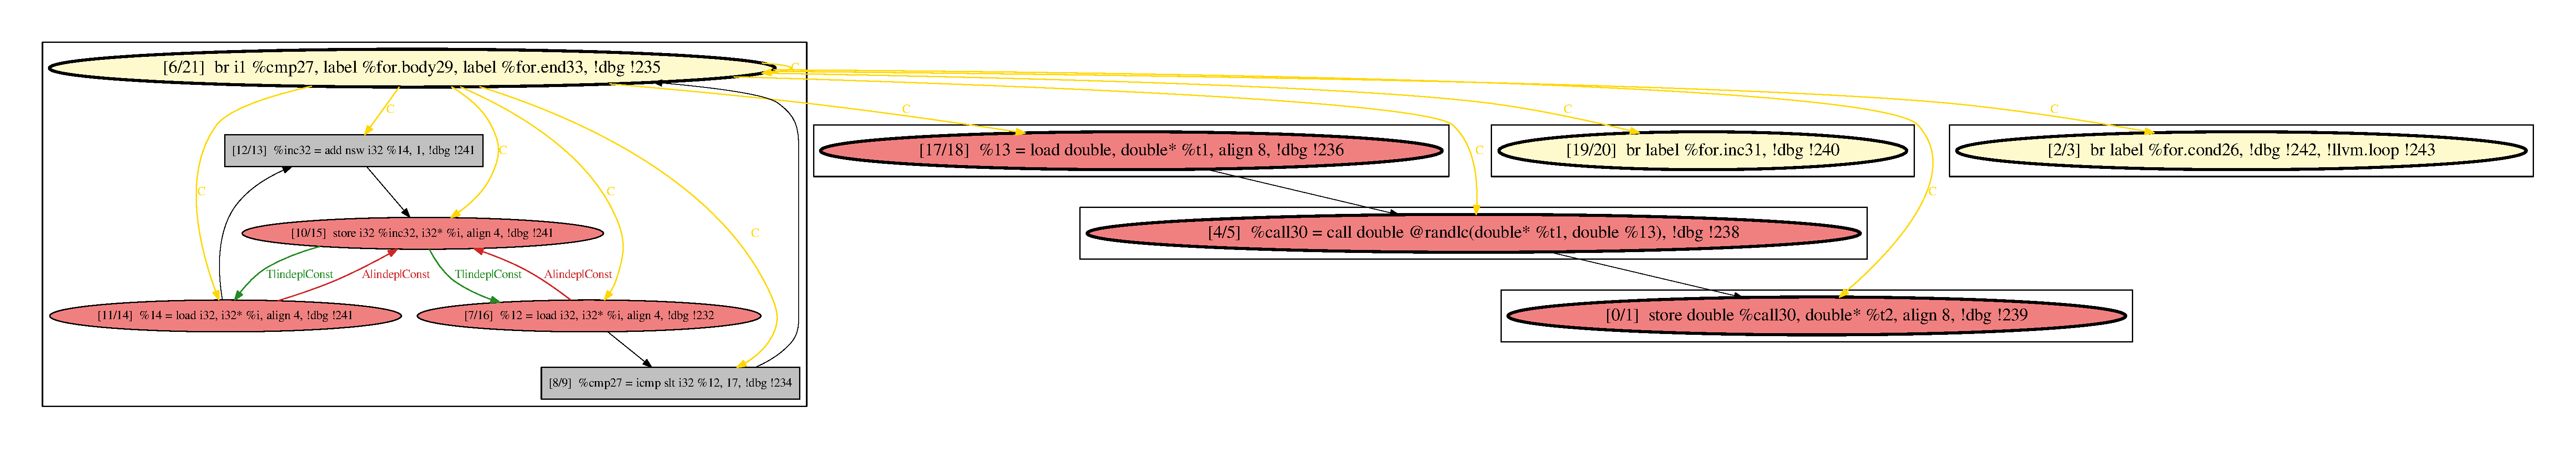
\includegraphics[width=\linewidth]{figs/metrics-example-loop-2-pdg.pdf}
	\caption{Program dependence graph (PDG) of the loop \ref{lst:metrics-loop-example-2}, as built and visualized by the PPar tool \ref{ppar-tool}.}
	\label{metrics-example-loop-2-pdg}
\end{figure}

\null\qquad Loop in the listing \ref{lst:metrics-loop-example-2} has a pretty simple PDG. There are no critical SCCs inside loop's payload. However, ICC compiler cannot parallelize this loop due to \textit{randlc} function call. Compiler has to be conservative and assume, that this function call introduces cross-iteration dependencies between iterations of the loop.\newline
\null\qquad This example exposes drawback of proper SCCs number metric. This metric only considers structural properties of PDG and does not examine the nature of instructions, constituting the loop. 


\section{Statistical analysis}
\label{analysis-statistical-analysis}
\qquad This section views loop parallelizability as a machine learning problem. Metrics represent features of loops. Intel C/C++ compiler gives an expert-opinion and labels (classifies) loops as parallelizible or not.
   
\qquad Statistical analysis of loop parallelisability metrics has been conducted with the help of pandas \cite{python-lib-pandas} and scikit-learn \cite{python-lib-scikit-learn} python packages. Detailed description of all algorithms, techniques and all underlying mathematical foundations can be found in the introduction to statistical analysis book \cite{statistical-learning-book}.

\subsection{K-Means clustering}

\qquad In this work k-means clustering techniques have been used as the first method of statistical analysis.




\subsection{SVM-based parallelisability analyzer}